%====================================================
% GBREK – LaTeX Beamer Template
%====================================================
\documentclass[aspectratio=169]{beamer} 

%-------------------------
% GENERAL PACKAGES
%-------------------------
\usepackage[utf8]{inputenc}
\usepackage[T1]{fontenc}
\usepackage{lmodern}          % nicer font
\usepackage{amsmath, amsfonts, amssymb}
\usepackage{bm}               % bold math
\usepackage{graphicx}
\usepackage{xcolor}
\usepackage{hyperref}
\usepackage{subcaption}
\usepackage{multirow}
\usepackage{booktabs}
\usepackage{subcaption} % recommended
% or: \usepackage{subfig}


% Optional: algorithm environment
\usepackage[ruled,vlined]{algorithm2e}

% \newtheorem{theorem}{Theorem}[section]
\newtheorem{proposition}[theorem]{Proposition}
% \newtheorem{corollary}[theorem]{Corollary}
% \newtheorem{example}[theorem]{Example}
\newtheorem{remark}[theorem]{Remark}
% \newtheorem{definition}[theorem]{Definition}
% \newtheorem{lemma}[theorem]{Lemma}


% --- calligraphic tensors ---
\newcommand{\mcalA}{\mathcal{A}}
\newcommand{\mcalB}{\fm B}
\newcommand{\mcalX}{\mathcal{X}}
\newcommand{\mcalZ}{\mathcal{Z}}
\newcommand{\mcalR}{\mathcal{R}}
\newcommand{\mcalO}{\mathcal{O}} % zero tensor (use \mcalO)

% --- sets / operators ---
\newcommand{\Null}{\mathrm{Null}}
\newcommand{\ran}{\mathrm{range}}




 
\def\l{\left} 
\def\r{\right} 
\def\mbf{\mathbf}

\def\rmf{{\rm F}}

\def\wh{\widehat}
\def\wt{\widetilde}

\def\bcirc{{\rm bcirc}}
\def\unfold{{\rm unfold}}
\def\fold{{\rm fold}} 
%\def\dia{{\rm diag}}
\def\rank{{\rm rank}} 
\def\ran{{\rm range}} 
\def\nul{{\rm null}}
\def\sgn{{\rm sgn}} 


\def\mcala{\mathcal A}
\def\mcalb{\mathcal B}
\def\mcalc{\mathcal C}
\def\mcale{\mathcal E}
%\def\mcalg{\mathcal G}
\def\mcali{\mathcal I}
\def\mcalw{\mathcal W}
\def\mcalx{\mathcal X}
\def\mcaly{\mathcal Y}
\def\mcalz{\mathcal Z}
\DeclareMathOperator*{\argmin}{argmin}

\def\mbbe{\mathbb E}
\def\mbbr{\mathbb R}

\def\dsp{\displaystyle} 
\def\nn{\nonumber}

\newcommand{\beq}{\begin{equation}}\newcommand{\eeq}{\end{equation}}
\newcommand{\bit}{\begin{itemize}}\newcommand{\eit}{\end{itemize}}
\newcommand{\bem}{\begin{bmatrix}}\newcommand{\eem}{\end{bmatrix}}



%-------------------------
% THEME & COLORS
%-------------------------
% \usetheme{Madrid}             % clean built-in theme
% \usecolortheme{dolphin}

% % Custom GBREK color palette
% \definecolor{GBREKBlue}{RGB}{0, 60, 130}   % main accent
% \definecolor{GBREKGreen}{RGB}{0, 150, 110} % secondary accent
% \definecolor{GBREKGray}{RGB}{245, 245, 245}

% % Apply colors
% \setbeamercolor{structure}{fg=GBREKBlue}
% \setbeamercolor{title}{fg=white,bg=GBREKBlue}
% \setbeamercolor{frametitle}{fg=white,bg=GBREKBlue}
% \setbeamercolor{block title}{fg=white,bg=GBREKGreen}
% \setbeamercolor{block body}{bg=GBREKGray}
% \setbeamercolor{itemize item}{fg=GBREKBlue}
% \setbeamercolor{itemize subitem}{fg=GBREKGreen}

% % Remove navigation symbols
% \setbeamertemplate{navigation symbols}{}

% % Footline with short title + page number
\setbeamertemplate{footline}{%
  \leavevmode%
  \hbox{%
    \begin{beamercolorbox}[wd=.8\paperwidth,ht=2.75ex,dp=1.25ex,left]{author in head/foot}%
      \usebeamerfont{author in head/foot}\hspace*{1em}\insertshorttitle
    \end{beamercolorbox}%
    \begin{beamercolorbox}[wd=.2\paperwidth,ht=2.75ex,dp=1.25ex,right]{date in head/foot}%
      \usebeamerfont{date in head/foot}\insertframenumber{} / \inserttotalframenumber\hspace*{1em}
    \end{beamercolorbox}}%
  \vskip0pt%
}

%-------------------------
% CUSTOM MACROS
%-------------------------
% \newcommand{\R}{\mathbb{R}}
\newcommand{\GBREK}{\text{GBREK}}



% --------personal commands ------
\def\fm#1{\mathcal{#1}}
\def\m#1{\boldsymbol{#1}}
\def\mb{\boldsymbol{\beta}}
\def\b{\beta}
\def\r{\mathbb{R}}
\def\tvx{\Tilde{\vx}}
\def\t#1{\Tilde{#1}}
\def\pr{Pr}
\def\EE{\mathbb{E}}
\def\Ukcol{\mathcal{U}^c_k}
\def\Ukrow{\mathcal{U}^r_k}
\def \ajk{\m A_{:, J_{j_k}}}
\def \aik{\m A_{I_{i_k}, :}}
\def \ai#1{\m A_{I_{#1}, :}}
\def \aj#1{\m A_{:,J_{#1}}}
\def\bik{\m b_{I_{k}}}
\def \bi#1{\m b_{I_{#1}}}
\def\zik{\m z_{I_{k}}}
\def\zi#1{\m z_{I_{#1}}}
% \def \xk#1#2{\m #1_{:, }}


% --------personal commands ------
\def\fm#1{\mathcal{#1}}
\def\m#1{\boldsymbol{#1}}
\def\mb{\boldsymbol{\beta}}
\def\b{\beta}
\def\r{\mathbb{R}}
\def\tvx{\Tilde{\vx}}
\def\t#1{\Tilde{#1}}
\def\pr{Pr}

\def \a#1{\fm A_{:, #1, :}}
\def \b#1{\fm B_{#1, :, :}}
\def \ai#1{\fm A_{#1, :, :}}
\def \z#1#2{\fm Z^{(#1)}_{#2, :, :}}
\def \bp#1{\fm B^{\perp}_{#1, :, :}}
\def \x#1{\fm X^{(#1)}}

% Short title & author for footer
\title[TGDBEK]{
    Solving Tensor Linear Systems  under the t-product by a Kaczmarz-type method
    }
\author[Jeremie Mabiala]{Jeremie Mabiala}
\institute[]{%
Kera Health, Inc.
}
\date{DTS 2026}
% Path to images (relative to this .tex file)
\graphicspath{{../../imgs/}}

%====================================================
\begin{document}
%====================================================

%-------------------------
% SLIDE 1: TITLE (30 s)
%-------------------------
\begin{frame}
  \titlepage
\end{frame}

%-------------------------
% SLIDE 2: MOTIVATION (1 min)
%-------------------------
\section{Motivation}
\begin{frame}{Why Tensors?}
  \begin{columns}[T]
    \begin{column}{0.55\textwidth}
      \begin{itemize}
        \item Images, videos, and multi-dimensional data are naturally represented as \textbf{third-order tensors}
              $\mcalA \in \mbbr^{m \times n \times p}$.
        \item \textbf{Image reconstruction}: given a blurred/noisy observation $\mcalB$,
              recover the clean image $\mcalX$ from
              \[
                \mcalA * \mcalX = \mcalB
              \]
              where $*$ denotes the \emph{t-product}.
        \item Systems are often \textbf{large-scale} and \textbf{inconsistent}.
      \end{itemize}
    \end{column}
    \begin{column}{0.4\textwidth}
      \centering
      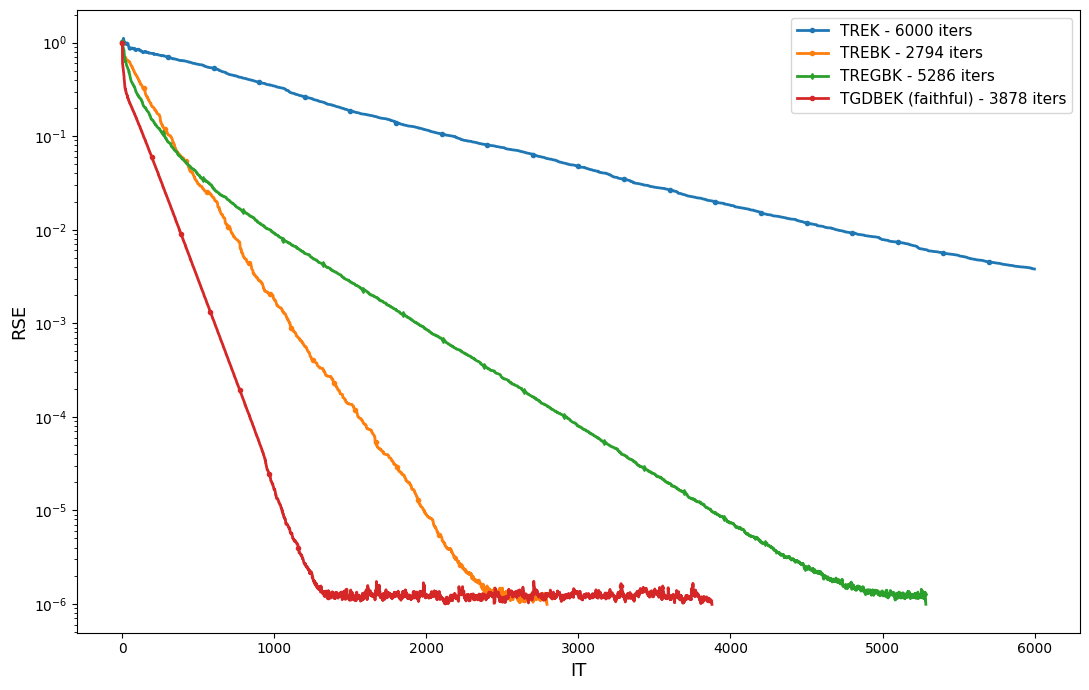
\includegraphics[width=\linewidth]{cities_tgdbek.png}
      \\[4pt]
      {\small Convergence on \texttt{Cities} matrix}
    \end{column}
  \end{columns}
\end{frame}

%-------------------------
% SLIDE 3: PROBLEM STATEMENT (1 min)
%-------------------------
\section{Problem Statement}
\begin{frame}{Problem Setup}
  \begin{block}{Tensor Linear System}
    Given $\mcalA \in \mbbr^{m \times n \times p}$ and $\mcalB \in \mbbr^{m \times k \times p}$,
    find $\mcalX \in \mbbr^{n \times k \times p}$ satisfying:
    \[
      \mcalA * \mcalX = \mcalB
    \]
  \end{block}

  \medskip
  \textbf{Goal:} compute the \emph{minimum-norm least-squares} solution
  \[
    \mcalX^{\star} = \argmin_{\mcalX} \| \mcalX \|_F
    \quad \text{s.t.} \quad
    \mcalX \in \argmin_{\mcalZ} \| \mcalA * \mcalZ - \mcalB \|_F
  \]

  \medskip
  \textbf{Setting:}
  \begin{itemize}
    \item System can be \textbf{inconsistent} ($\mcalB \notin \ran(\mcalA)$)
    \item Dimensions $m, n$ large $\Rightarrow$ direct solvers impractical
    \item Iterative Kaczmarz-type methods are well-suited
  \end{itemize}
\end{frame}

%-------------------------
% SLIDE 4: EXISTING METHODS & GAPS (1 min)
%-------------------------
\section{Related Work}
\begin{frame}{Existing Methods \& Limitations}
  \textbf{Tensor Kaczmarz variants in the literature:}
  \begin{itemize}
    \item \textbf{TREK} -- Tensor Randomized Extended Kaczmarz
    \item \textbf{TREBK} -- Tensor Randomized Extended Block Kaczmarz
    \item \textbf{TREGBK} -- Tensor Randomized Extended Greedy Block Kaczmarz
  \end{itemize}

  \bigskip
  \textbf{Key limitation:}
  \begin{alertblock}{Pre-defined Partitions Required}
    TREBK, TREGBK, and similar block methods require a
    \textbf{pre-defined partition} of the row/column indices.
    \begin{itemize}
      \item Partition quality directly affects convergence
      \item No principled way to choose the partition a priori
      \item Extra tuning overhead
    \end{itemize}
  \end{alertblock}
\end{frame}

%-------------------------
% SLIDE 5: TGDBEK KEY IDEA (1.5 min)
%-------------------------
\section{Proposed Method: TGDBEK}
\begin{frame}{TGDBEK: Key Idea}
  \begin{columns}[T]
    \begin{column}{0.52\textwidth}
      \textbf{Two-step greedy selection} at each iteration $k$:

      \medskip
      \textbf{Z-step} (column selection):
      \begin{itemize}
        \item Score each column slice by its contribution
        \item Greedily select the set $U_k$ of most informative columns
        \item Project: $\mcalZ^{k+1} \leftarrow \mcalZ^{k} - \mcalA_{:,U_k,:} * (\mcalA_{:,U_k,:})^{\dagger} * \mcalZ^{k}$
      \end{itemize}

      \medskip
      \textbf{X-step} (row selection):
      \begin{itemize}
        \item Score each row slice by its residual
        \item Greedily select the set $J_k$ of most informative rows
        \item Update: $\mcalX^{k+1} \leftarrow \mcalX^{k} + (\mcalA_{J_k,:,:})^{\dagger} * \mcalR_{J_k}$
      \end{itemize}

      \medskip
      \textbf{No pre-defined partitions needed!}
    \end{column}
    \begin{column}{0.45\textwidth}
      \centering
      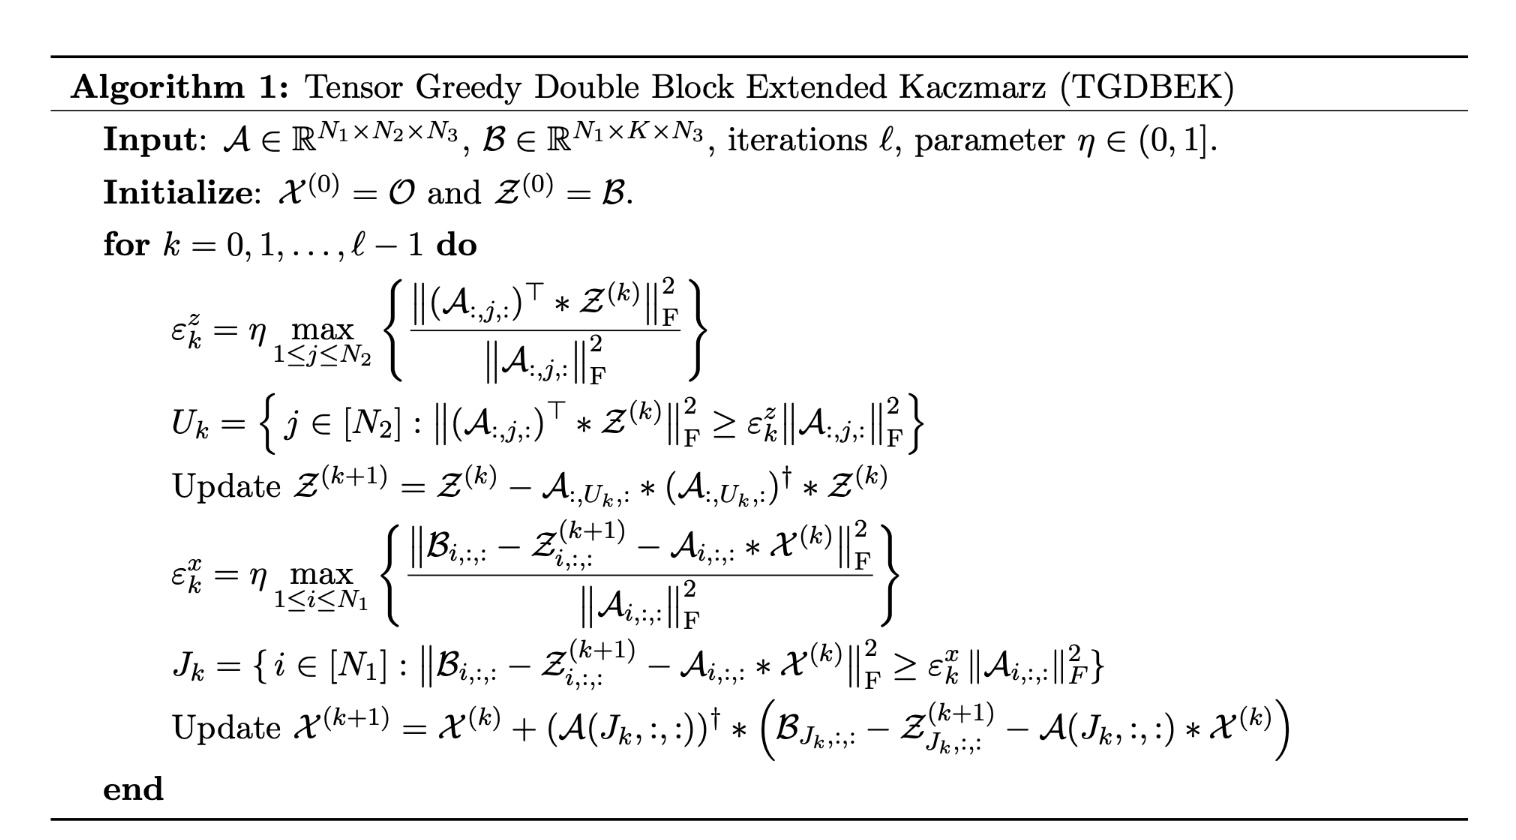
\includegraphics[width=\linewidth]{tgdbek_algorithm.jpg}
      \\[4pt]
      {\small The TGDBEK Algorithm}
    \end{column}
  \end{columns}
\end{frame}

%-------------------------
% SLIDE 6: GREEDY SELECTION DETAIL (1 min)
%-------------------------
\begin{frame}[shrink=10]{Greedy Selection Criterion}
  \small
  Given a parameter $\eta \in (0, 1]$:

  \smallskip
  \textbf{Column selection (Z-step):}
  \[
    \varepsilon_z^k = \eta \cdot \max_j
    \frac{\| (\mcalA_{:,j,:})^\top * \mcalZ^k \|_F^2}{\| \mcalA_{:,j,:} \|_F^2},
    \quad
    U_k = \Big\{ j :
    \frac{\| (\mcalA_{:,j,:})^\top * \mcalZ^k \|_F^2}{\| \mcalA_{:,j,:} \|_F^2}
    \geq \varepsilon_z^k \Big\}
  \]

  \smallskip
  \textbf{Row selection (X-step):}
  \[
    \varepsilon_x^k = \eta \cdot \max_i
    \frac{\| \mcalB_{i,:,:} - \mcalZ^{k+1}_{i,:,:} - \mcalA_{i,:,:} * \mcalX^k \|_F^2}{\| \mcalA_{i,:,:} \|_F^2},
    \quad
    J_k = \Big\{ i : \text{score}_i \geq \varepsilon_x^k \Big\}
  \]

  \smallskip
  \begin{itemize}
    \item $\eta \to 1$: fewer, most informative slices (aggressive)
    \item $\eta \to 0$: more slices selected (conservative)
    \item $U_k, J_k$ are \textbf{determined adaptively} at each iteration
  \end{itemize}
\end{frame}

%-------------------------
% SLIDE 7: CONVERGENCE (1 min)
%-------------------------
\section{Convergence}
\begin{frame}{Convergence Guarantee}
  \begin{theorem}
    Let $\mcalA \in \mbbr^{m \times n \times p}$ and $\mcalB \in \mbbr^{m \times k \times p}$.
    The iterates $\{\mcalX^k\}$ produced by TGDBEK converge \textbf{linearly} to the
    minimum-norm least-squares solution $\mcalX^{\star}$:
    \[
      \mbbe\big[\| \mcalX^k - \mcalX^{\star} \|_F^2\big]
      \;\leq\;
      \rho^k \, \| \mcalX^0 - \mcalX^{\star} \|_F^2
    \]
    where $0 < \rho < 1$ depends on $\eta$ and the spectral properties of $\mcalA$.
  \end{theorem}

  \medskip
  \textbf{Key points:}
  \begin{itemize}
    \item Convergence to the \emph{minimum-norm least-squares} solution
    \item Works for inconsistent systems
    \item Rate improves with well-conditioned $\mcalA$ and appropriate $\eta$
  \end{itemize}

  \vfill
  {\small \textit{Full proof available in the technical report.}}
\end{frame}

%-------------------------
% SLIDE 8: NUMERICAL RESULTS (1.5 min)
%-------------------------
\section{Numerical Experiments}
\begin{frame}[shrink=10]{Results on Sparse Matrices (SuiteSparse)}
  \small
  \begin{columns}[T]
    \begin{column}{0.52\textwidth}
      \centering
      {\small \textbf{ash85} ($85 \times 85$, density $= 0.072$)}

      \smallskip
      \begin{tabular}{@{}lrrr@{}}
        \toprule
        \textbf{Method} & \textbf{Time} & \textbf{RSE} & \textbf{IT} \\
        \midrule
        TREK    & 0.370 & $2.0\mathrm{e}{-2}$  & 500 \\
        TREBK   & 0.369 & $9.2\mathrm{e}{-7}$  & 174 \\
        TREGBK  & 0.574 & $9.9\mathrm{e}{-7}$  & 258 \\
        \textbf{TGDBEK} & \textbf{0.248} & $9.3\mathrm{e}{-7}$ & \textbf{78} \\
        \bottomrule
      \end{tabular}

      \medskip
      {\small \textbf{nos5} ($153 \times 153$, density $= 0.047$)}

      \smallskip
      \begin{tabular}{@{}lrrr@{}}
        \toprule
        \textbf{Method} & \textbf{Time} & \textbf{RSE} & \textbf{IT} \\
        \midrule
        TREK    & 0.454 & $1.0\mathrm{e}{-1}$ & 300 \\
        TREBK   & 0.860 & $9.8\mathrm{e}{-7}$ & 144 \\
        TREGBK  & 0.864 & $9.9\mathrm{e}{-7}$ & 124 \\
        \textbf{TGDBEK} & \textbf{0.581} & $9.7\mathrm{e}{-7}$ & \textbf{45} \\
        \bottomrule
      \end{tabular}
    \end{column}
    \begin{column}{0.45\textwidth}
      \centering
      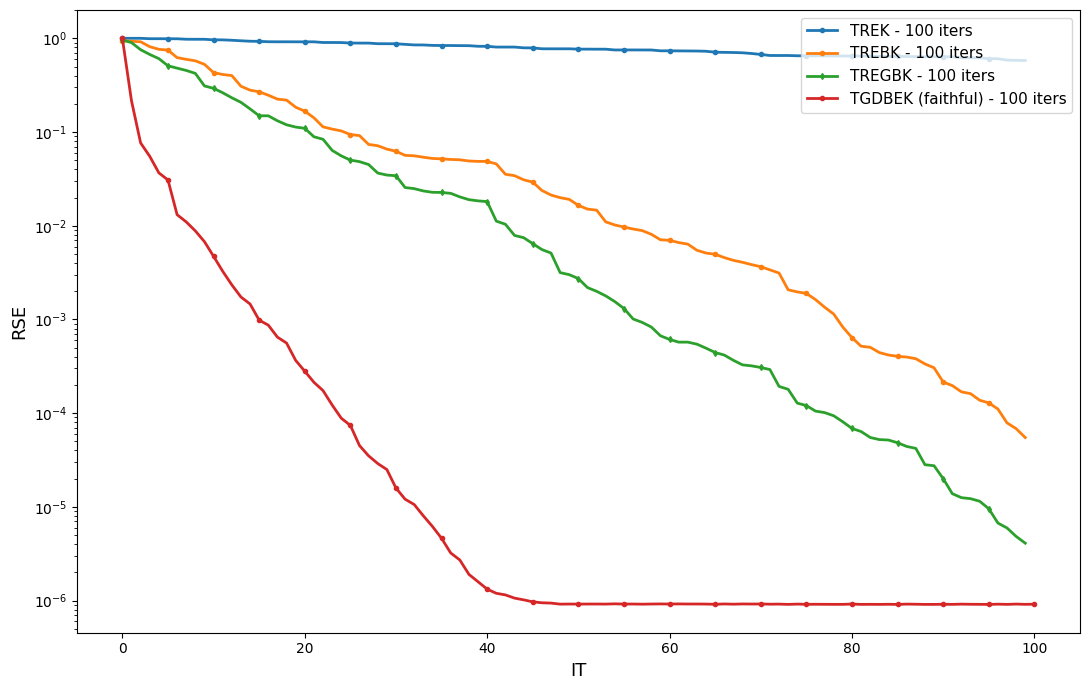
\includegraphics[width=\linewidth]{ash85_tdgbek.png}
      \\[1pt]
      {\scriptsize RSE vs.\ Iterations (ash85)}

      \medskip
      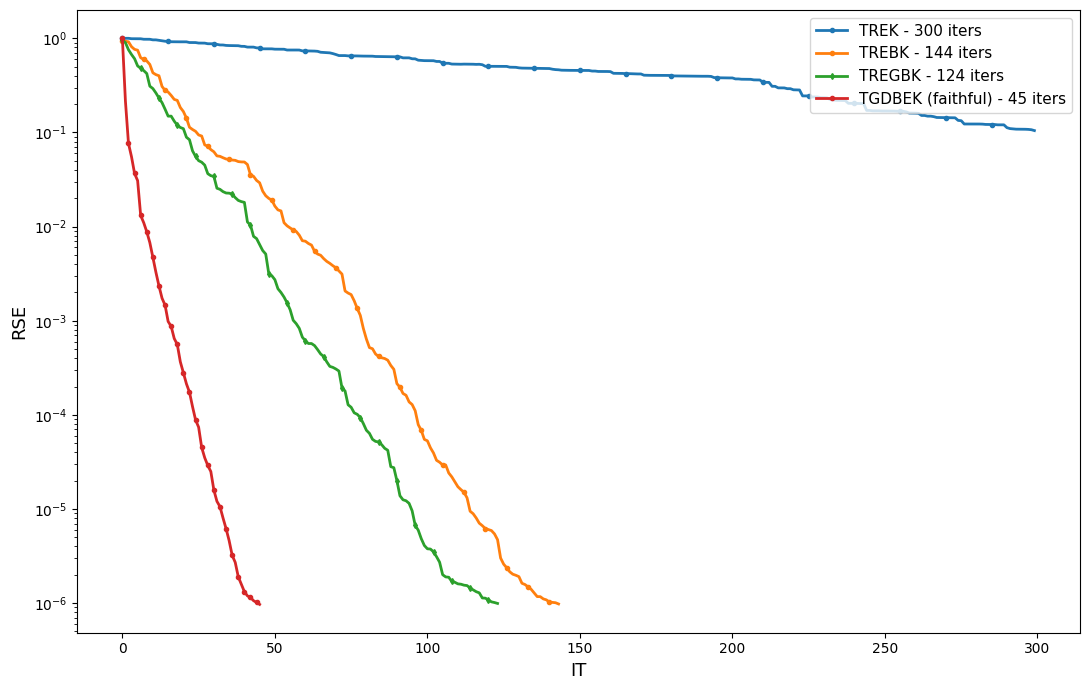
\includegraphics[width=\linewidth]{nos5_tdgbek.png}
      \\[1pt]
      {\scriptsize RSE vs.\ Iterations (nos5)}
    \end{column}
  \end{columns}
\end{frame}

%-------------------------
% SLIDE 9: MORE RESULTS -- CITIES (30 s)
%-------------------------
\begin{frame}{Results: Cities Matrix ($128 \times 128$)}
  \begin{columns}[c]
    \begin{column}{0.5\textwidth}
      \centering
      \begin{tabular}{@{}lrrr@{}}
        \toprule
        \textbf{Method} & \textbf{Time} & \textbf{RSE} & \textbf{IT} \\
        \midrule
        TREK    & 4.089 & $3.8\mathrm{e}{-3}$ & 6000 \\
        TREBK   & 3.318 & $9.9\mathrm{e}{-7}$ & 2794 \\
        TREGBK  & 6.943 & $9.9\mathrm{e}{-7}$ & 5286 \\
        \textbf{TGDBEK} & 5.954 & $9.9\mathrm{e}{-7}$ & \textbf{3878} \\
        \bottomrule
      \end{tabular}
    \end{column}
    \begin{column}{0.45\textwidth}
      \centering
      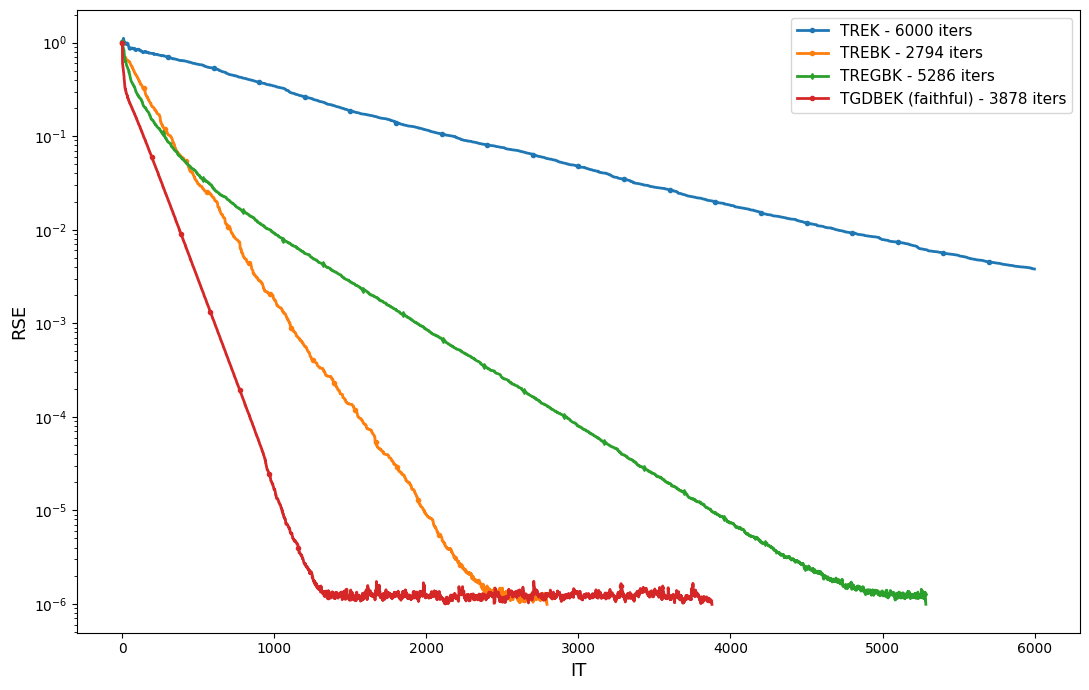
\includegraphics[width=\linewidth]{cities_tgdbek.png}
      \\[4pt]
      {\small RSE vs.\ Iterations (Cities)}
    \end{column}
  \end{columns}

  \bigskip
  \textbf{Takeaway:}
  \begin{itemize}
    \item TGDBEK consistently reaches target accuracy with \textbf{fewer iterations}
    \item Competitive or better wall-clock time \textbf{without needing partition tuning}
  \end{itemize}
\end{frame}

%-------------------------
% SLIDE 10: SUMMARY & FUTURE WORK (1 min)
%-------------------------
\section{Conclusion}
\begin{frame}{Summary \& Future Work}
  \textbf{Summary:}
  \begin{enumerate}
    \item \textbf{No pre-defined partitions} -- greedy selection adapts at each step
    \item \textbf{Faster convergence} -- fewer iterations than TREK, TREBK, TREGBK
    \item \textbf{Proven guarantees} -- linear convergence to min-norm LS solution
  \end{enumerate}

  \bigskip
  \textbf{Future work:}
  \begin{itemize}
    \item Larger-scale experiments (high-resolution images, video)
    \item GPU-accelerated implementation via PyTorch
    \item Extensions to other tensor decompositions (Tucker, TT)
    \item Applications to tensor completion and compressed sensing
  \end{itemize}

  \bigskip
  \begin{center}
    \textbf{Thank you!}
    \\[6pt]
    Code: \url{https://github.com/jnlandu/tensor-greedy-double-extended-kaczmarz}
  \end{center}
\end{frame}

\end{document}